
\section*{Introduction}%prevent numbering for the intro
\addcontentsline{toc}{section}{\protect\numberline{}\hspace{0.3cm}Introduction}%add intro to contents

The first viable \textit{inorganic} solar cells came to light at Bell~Laboratories in 1954 \cite{siliconSC_1}\cite{siliconSC_2} with power conversion efficiencies of about 6 percent. Though the commercial success was limited because of high production costs, Chapin, Pearson and Fuller proved to us that it is possible to harness significant amounts of solar energy for practical usage and thus set foot for photovoltaic advancements.\mypar
Today's challenge is however to build low-cost solar cells that can be tailored to their specific application and can be produced in large amounts with established manufacturing processes\footnote{For an example of a realized roll-to-roll production see \cite{rolltoroll}.}. This has lead us to \textbf{organic} solar cells (\OSC).\mypar
Because of low efficiencies of heterojunction solar cells developed in the 1980s \cite{tang}, new concepts arose like the >>bulk~heterojunction<< (\BHJ) solar cell \cite{heterojunk}. It promised to bypass the problem of the short diffusion length of excitons created in the heterojunction as well as the limited thickness of the junction layers in a heterojunction cell.\mypar
Bulk heterojunction solar cells (\BHSC) still stand as state of the art technology as they are subject of current research (see~\cite{modernbulkhetero}). In this lab course we went through the process of assembling 5 different sets $\mathbb{S}_k$ of \BHSC\ and characterized them with the {\os\sefo AM 1.5} global reference spectrum. In the following we will review the assembly\footnote{We will call it assembly because we did not perform the complete preparation of all used materials.} and evaluate the obtained $I$-$U$-curves.

\section{Assembly of bulk heterojunction solar cells}\label{sec:assembly}
For each of the 5 sets of \BHSC's we performed all steps of the assembly on square glass substrates with sides of approximately 2~cm. The used substrates were coated with two ITO stripes (see \cite{labdesc} Figure~12) with a width of
\begin{equation*}
w = (1600\pm50)\;\text{\textmu m}.
\end{equation*}
Where we assumed a measurement uncertainty of an analog caliper. The viewing-angle-dependent visibility of the transparent ITO stripes, created the necessity of a shallow scratch on the glass. This helped identifying the orientation of the substrates later on.\mypar
We followed the assembly procedure given to us in Section~3.5 of \cite{labdesc}. After the removal of any remaining residue on the glass substrates, we applied the active layers onto them via spin coating and annealing afterwards. Finally aluminum cathodes were applied by thermal evaporation. On two sets we prepared drops of Galinstan as cathodes that we applied with syringes.

\subsection{Thermal evaporation}\label{subsec:therm-eva}
When we had annealed all active layers onto all substrates we let them cool down and put $\mathbb{S}_1$, $\mathbb{S}_2$ and $\mathbb{S}_4$ into a vacuum chamber. Sets $\mathbb{S}_3$ and $\mathbb{S}_5$ were left outside in a petri dish covered with aluminum foil. The chamber was pumped down to a pressure of $p_0 = (3.6\pm 0.1)\cdot 10^{-8}\; \mathrm{mbar}$ over 4 days and 15 hours.\mypar
We began heating up the aluminum filament by increasing the current flowing through it in steps of around 5~A. The small step sizes ensured the protection of the filament as we had to reach currents above 30~A. Because of the increasing temperature of the filament, gases trapped inside it and in it's surroundings exited into the chamber. So each time we increased the current flow, the pressure increased significantly and slowly decreased in the following as the pump continued to run. Between each current increase, we waited until the pressure had stabilized. As we approached a current of around 23~A, the filaments incandescent glow was visible and we positioned all sets contained in the chamber directly above the filament. At this point the pressure increased up to around $8.6p_0$ and increased further to $30.5p_0$ as we reached a current of 30~A.\mypar
The sets were mounted into a sample holder with a mask. That way, evaporated aluminum could only condensate on the exposed sample surfaces in the way shown in \cite{labdesc} Figure 12. To achieve the right orientation the ITO stripes mentioned above, had to be perpendicular to the mask of the sample holder. Unfortunately we did not get the right orientation on sets $\mathbb{S}_1$ and $\mathbb{S}_2$ and the aluminum cathodes condensated in an orientation parallel to the ITO stripes. This forced us to use Galinstan cathodes on sets $\mathbb{S}_1$ and $\mathbb{S}_2$ but because of the \emph{now} small space left on the substrate we created a short circuit on set $\mathbb{S}_2$ in the process.

\subsection{Active area with Galinstan cathode}

To obtain current densities $j(U)$ in Section~\ref{sec:charac} we will need the active area $A_{kn}$ of a cell $n$ of the set $\mathbb{S}_k$. As the majority of our assembled cells had Galinstan cathodes we will have a detailed look into the determination of $A_{kn}$. We will drop the index $k$ in order to maintain a clear notation.\mypar
As for an aluminum cathode (see \cite{labdesc} Figure 12) we will assume the active area is defined as the visible overlap

\begin{figure}[H]\centering
\subimport{../1_Pictures/}{Blobs.pdf_tex}
\caption{Top-down view of an assembled set of \BHSC's with spherical assumed Galinstan cathode. An active area $A_n$ of a cell of this set is highlighted in blue. }
\label{fig:blobs}
\end{figure}

\clearpage

\onecolumn
\begin{table}[t]\centering
\caption{Overview of intended and achieved architectures of the assembled sets. $N$ refers to the total numbers of cells prepared on this set and $N_\checkmark$ refers to the number of cells that came out to \emph{not} have a short circuit. Set $\mathbb{S}_\star$ denotes the set of \BHSC's that was prepared by our supervisor.}
\label{tab:assemb-table}
\begin{tabular}{@{}c|ccccccc@{}}\toprule\toprule
Set                             && $\mathbb{S}_1$ & $\mathbb{S}_2$ & $\mathbb{S}_3$ & $\mathbb{S}_4$ & $\mathbb{S}_5$ & $\mathbb{S}_\star$ \\[2ex] %\cmidrule{2-7}
\multirow{4}{*}{Intended arch.} && ITO            & ITO            &                &                & PEIE           &                    \\
&& PEDOT:PSS      & PEDOT:PSS      &                &                & P3HT:PCBM      &                    \\
&& P3HT:PCBM      & P3HT:2PCBM     & \multirow{2}{*}{ITO}            &                & PEDOT:PSS      & \multirow{2}{*}{ITO}                \\
&& Aluminum       & Aluminum       & \multirow{2}{*}{PEDOT:PSS}      & ITO            & Galinstan      & \multirow{2}{*}{PEDOT:PSS}          \\
&&                &                & \multirow{2}{*}{P3HT:PCBM}      & P3HT:PCBM      &                & \multirow{2}{*}{P3HT:PCBM}          \\
\multirow{4}{*}{Achieved arch.} && ITO            & ITO            & \multirow{2}{*}{Galinstan}      & Aluminum       & PEIE           & \multirow{2}{*}{Galinstan}          \\
&& PEDOT:PSS      & PEDOT:PSS      &                &                & P3HT:PCBM      &                    \\
&& P3HT:PCBM      & P3HT:2PCBM     &                &                & Galinstan      &                    \\
&& Galinstan      & Galinstan      &                &                &                &                    \\
$N$                             && 2              & 2              & 5              & 4              & 5              & 4                  \\
$N_\checkmark$                  && 1              & 0              & 4              & 0              & 0              & 4                  \\ \bottomrule
\end{tabular}
\end{table}

\begin{figure}[t]\centering
\begin{minipage}{0.48\textwidth}\centering
\def\svgwidth{0.9\textwidth}
\caption{Assembled set $\mathbb{S}_5$ of \BHSC’s with a ruler next to it to translate the scale. $d_n^y$ and $d_n^x$ are indicated.}
\label{fig:realblob}
\subimport{../1_Pictures/}{cell5.pdf_tex}
\end{minipage}
\hspace{4mm}
\begin{minipage}{0.48\textwidth}\centering
\vspace*{-1.5\baselineskip}
\captionof{table}{Overview of all \emph{working} cells and their active areas $A_{kn}$. For set $\mathbb{S}_\star$ we used the average active area of all cells we documented.}
\begin{tabular}{@{}ccc@{}}\toprule
Set                             & Cell $n$ & $A_{kn}$ {[}mm$^2${]}     \\ \midrule
$\mathbb{S}_1$                  & 1        & 60.0(20)                  \\
&          &                           \\
\multirow{4}{*}{$\mathbb{S}_3$} & 2        & 58.4(20)                  \\
& 3        & 63.2(21)                  \\
& 4        & 59.2(20)                  \\
& 5        & 64.8(22)                  \\
&          &                           \\
$\mathbb{S}_\star$              & -        & $A_\star = 64.0(21)$ \\ \bottomrule
\end{tabular}
\end{minipage}
\end{figure}

\begin{multicols}{2}

of cathode and corresponding ITO stripe. Furthermore we assume that the Galinstan drop satisfies a spherical shape with diameter $\overline{d}_n$ and lies in the center of the ITO stripe. This leads to the geometry illustrated in Figure~\ref{fig:blobs} with the following expression for the active area
\begin{equation}\label{eq:blobarea}
A_n({\overline{d}_n}) = \frac{1}{2} \Bigg[ {\overline{d}_n}^2 \arcsin\left(\frac{w}{{\overline{d}_n}}\right) + w \sqrt{{\overline{d}_n}^2 - w^2} \Bigg].
\end{equation}

To obtain $\overline{d}_n$, we measured $d_n^x$ and $d_n^y$ by using pictures of the sets for which an example is shown in Figure~\ref{fig:realblob}. With the ruler in the picture we translated the scale $\Sigma^\prime$ of a screen projecting the image to the real scale $\Sigma$ of the cathode\footnote{A variable $x$ refers to scale $\Sigma$ and analogously $x^\prime$ refers to scale $\Sigma^\prime$}.\mypar
First we extracted the conversion factor $a$ which translates $\Sigma^\prime$ to $\Sigma$. This is done by measuring the length $x_0^\prime$ that is equivalent to a length $x_0$ we could read from the ruler in the picture. We assumed the uncertainty $u_{x_0^\prime}$ of half a division of \emph{the ruler we put on the screen}. And we assumed the uncertainty $u_{x_0}$ to be a third of a division, because of the magnification of \emph{the ruler that is visible} in Figure~\ref{fig:realblob}.
\begin{equation*}
u_{x_0^\prime} = 0.5 \;\mathrm{mm} \qquad u_{x_0} = 0.3 \;\mathrm{mm}
\end{equation*}
The factor $a$ and its relative uncertainty are then given by
\begin{equation}\label{eq:auncert}
a=\frac{x_0}{x_0^\prime} \quad \text{and} \quad \frac{u_a}{a} = \sqrt{\frac{{u_{x_0}}^2}{{x_0}^2}+\frac{{u_{x_0^\prime}}^2}{{x_0^\prime}^2}}\;.
\end{equation}

Any length $x^\prime$ of scale $\Sigma^\prime$ will now translate into the real length $x = a x^\prime$ with a relative uncertainty $u_x/x$ that is of the same form as in equation~\ref{eq:auncert} for $a$.\mypar
By this method for each picture and its conversion factor $a$ we obtained the diameters $d^x_n$ and $d^y_n$ for each cell. The diameter $\overline{d}_n$ that was used in equation~\ref{eq:blobarea} then resulted in
\begin{equation}
\overline{d}_n = \frac{1}{2} (d_n^x + d_n^y ).
\end{equation}

\end{multicols}

\clearpage
\twocolumn

\subsection{Description of set lineup}
As we continued to work on the assembly of all sets of \BHSC's, we encountered unforeseen deviations from our original plan of construction that resulted in different final architectures. For each set $\mathbb{S}_k$ we will describe the deviations and how they came to be. Table~\ref{tab:assemb-table} gives a summary of the assembly process.\mypar
In the previous section~\ref{subsec:therm-eva} we elaborated that set $\mathbb{S}_1$ and $\mathbb{S}_2$ were unfortunately equipped with aluminum cathodes with the wrong orientation. We tried to recover minimal functionality by applying Galinstan cathodes to both sets. This resulted in a short circuits for $\mathbb{S}_2$ and in one functional cell on set $\mathbb{S}_1$.\mypar
Set $\mathbb{S}_3$ and $\mathbb{S}_5$ were set aside during the evaporation process. As we prepared the Galinstan cathodes on $\mathbb{S}_3$ originally six cells were prepared but two of the cells merged, resulting in a significantly bigger cell that turned out to be shorted.

\begin{figure}[h]\centering
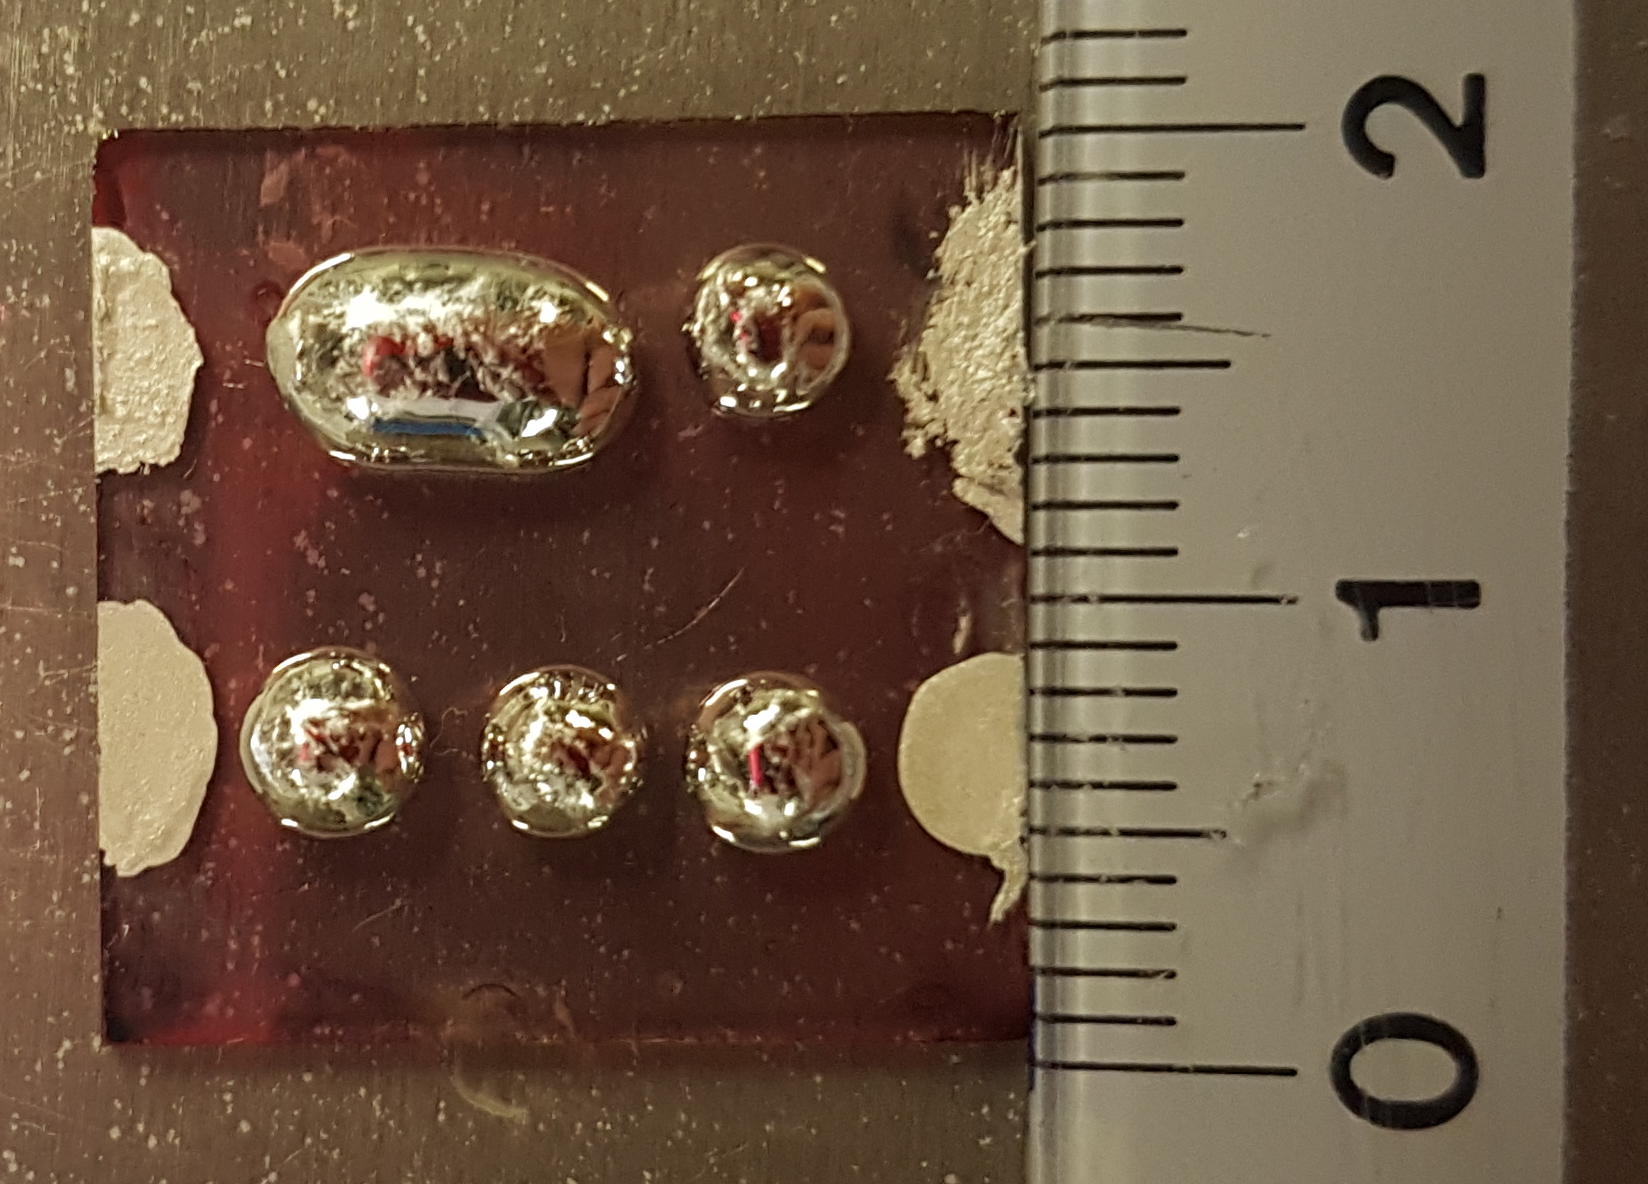
\includegraphics[width=0.9\columnwidth]{../1_Pictures/cell3.png}
\caption{Assembled set $\mathbb{S}_3$ with ruler next to it. Clearly visible are the two merged cells that became one big cell.}
\end{figure}
Set $\mathbb{S}_5$ underwent a special treatment as we tried to construct a unique architecture on it. The PEIE (electron injection) layer was applied first in contrast to PEDOT:PSS on all other sets. We wanted to apply PEDOT:PSS as the final layer but as it turns out this was not compatible with the properties of the surface of the annealed P3HT:PCBM layer. Tests of spin coating the aqueous solution of PEDOT:PSS onto the presumably hydrophobic P3HT:PCBM layer failed on set $\mathbb{S}_5$.\mypar
We accomplished the intended architecture on set $\mathbb{S}_4$ but when characterizing $\mathbb{S}_4$ turned out to be shorted.

